\subsection{HumanEvalFix Evaluation}
\label{appx:analyses:additional_benchmarks}
In this section, we include further discussion about our evaluation of SWE-agent on HumanEvalFix.
We choose to evaluate on the HumanEvalFix task because it focuses on code editing and debugging, which was empirically demonstrated in \citet{muennighoff2023octopack} to be a more difficult task for LMs (as reported in their work, GPT 4 scores \num{78.3}\% on HumanEval, compared to \num{47.8}\% on HumanEvalFix).
The code editing task can also be thought of as a ``subtask" in SWE-bench; being able to identify and fix bugs is a major part of software engineering.

We adopt the HumanEvalFix dataset (\num{164} problems per language) to be compatible with the SWE-agent setting.
Following the documentation in \citet{muennighoff2023octopack}, SWE-agent is initialized in a directory with a single file containing a buggy code snippet and example test(s) if available.
It is then asked to edit the code and verify its fixes.
The configuration file is identical to the one used for SWE-bench, with the exception of a language-specific demonstration.
For this task, localization and navigating a large codebase are not necessary; the main focus is on generating the correct edit.
SWE-agent achieves the best performance on the HumanEvalFix benchmark for three of the languages we evaluate on, as shown in Table~\ref{tab.benchmark_humanevalfix}.
Figure~\ref{fig.humanevalfix_dist_of_turns} also suggests that the large majority of task instances are solved within the first \num{10} turns.

\begin{figure}[ht]
    \centering
    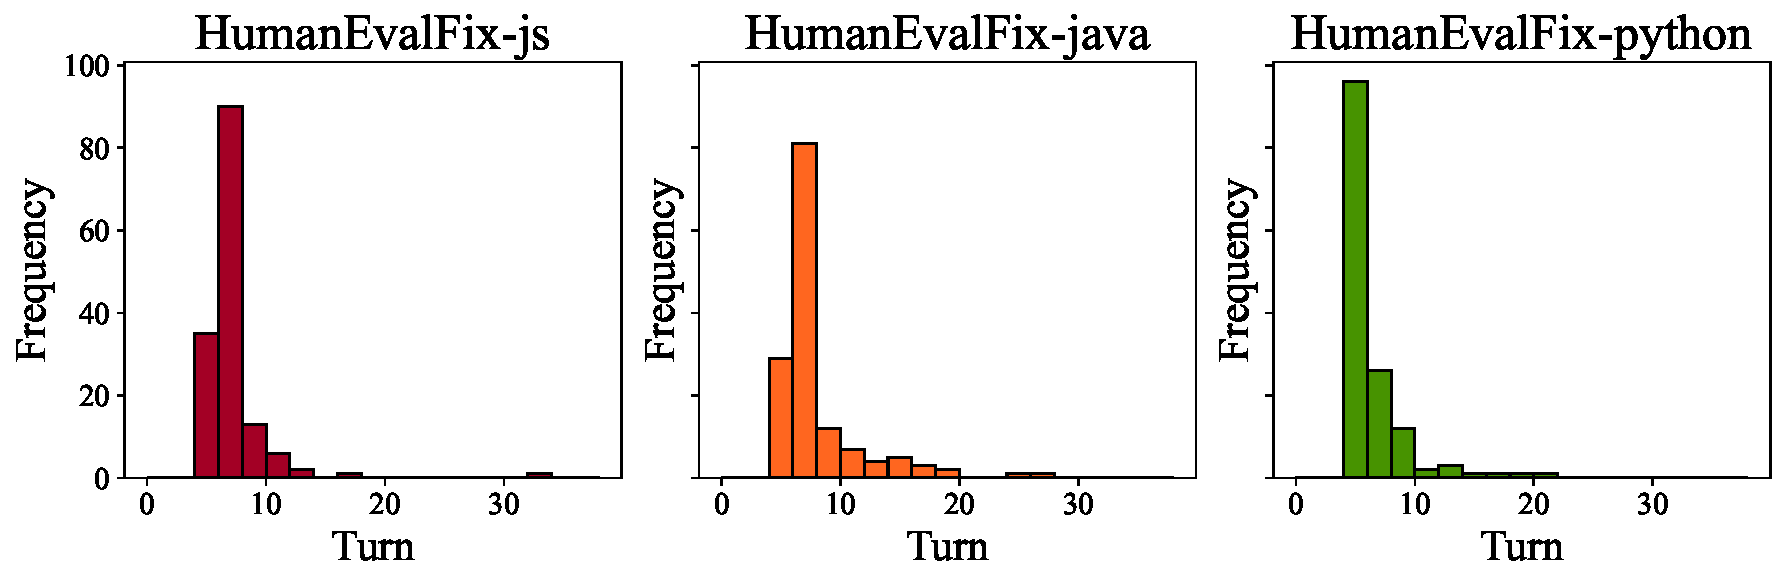
\includegraphics[width=\textwidth]{figures/appx/humanevalfix_turns.pdf}
    \caption{Similar to Figure~\ref{fig.resolved_by_turn}, we show the distribution of the number of turns for trajectories corersponding to solved task instances from the HumanEvalFix dataset.}
    \label{fig.humanevalfix_dist_of_turns}
\end{figure}